\section{On-chip Network}

%\subsection{Communication Patterns on Spatial Data-flow Accelerators}
%Unlike traditional processor-based architectures, where applications are executed in time and communication only occurs when accessing overlapping shared address space, communications on spatial architectures differ fundamentally in the following ways:
This section discusses communication characteristics common in
applications that have been spatially mapped to CGRAs. %In this paper, we explore a wide variety of interconnection network designs for CGRAs.
Because CGRAs encompass a broad range of architectures, we first describe the abstract machine model
of our target CGRA for this study, shown in  Figure~\ref{fig:arch}.
The CGRA contains Physical Units (PUs) corresponding to distributed hardware resources, including compute units, scratchpads, and DRAM controllers.
The communication between PUs, sent over a reconfigurable network, is purely streaming.
Compute PUs have a simple control mechanism: they wait on input data dependencies and stall for backpressure from the network. 
%The compute can have simple state machine allow rate matching between dependencies.
The network guarantees exactly-once, in-order delivery with variable latency, and communication between PUs can have varying granularities (e.g., 512-bit vector or 32-bit scalar).

%\subsection{CGRA Characteristics} 
In this study, we focus on two categories of CGRA architectures.
The first architecture uses pipelining in compute PUs, as shown in Figure~\ref{fig:arch}.
To provide high throughput, each stage of the pipeline exploits SIMD parallelism, and multiple SIMD operations are pipelined within a PU.
Plasticine, a recently proposed CGRA, is an example of a pipelined architecture \cite{plasticine}.
%Since computations are laid out in space, pipelined communication forms between data producers and consumers.  
%Due to the pipelined computation, performance is less sensitive to the latency of the communication. 
%Therefore, high-bandwidth network resource such as static network, is required to sustain throughput of the application. 
%Elsewhere, coarse-grained pipelines introduce communications that are far less frequent; these include loading data from DRAM to on-chip SRAMs.
%Example of coarse-grained communication includes initialization of the on-chip memory where off-chip load and on-chip compute are overlapped to hide DRAM latency, and reading of loop invariant variables from inner loop pipeline. 
%The network requirements depend on the pipeline granularity. 
%In the case of fine-grained pipelining, which happens if the long body of an inner-most loop is mapped across different computation tiles, the communication occurs every cycle and is highly throughput (but not latency) sensitive.
%Such communications are tolerant of lower network throughput, which reveals the opportunity of link sharing.

%\subsubsection{Time-Shared Computation}
%Instead of spreading a computation over multiple compute units, it is also possible to distribute it over several cycles:
%in such a CGRA, variables are not loaded into each compute unit every cycle.
%By keeping more computation in a single compute unit, the total amount of network communication is reduced and there are more opportunities for link sharing than with the pipelined network.
%Figure~\ref{fig:link}(a) shows the activation rate of all communications in the program. About 40\% of the links are firing at more than 50\% of the time for most of the compute bound applications, such as GDA, GEMM, and Kmeans. On the other hand, about half of the links activate at very low frequency, where link sharing can improve overall link utilization.
The second architecture uses time-scheduled execution, where each PU executes a small loop of instructions (e.g., 6) repeatedly. 
The scheduling window is small enough that instructions are stored as part of the configuration fabric, without dynamic instruction fetch overhead. 
This execution model creates more interleaved pipelining across PUs with communication that is tolerant of lower network throughput, which provides an opportunity to share links.
Many proposed CGRAs and domain-specific architectures use this \emph{time-scheduled} form of computation, including Brainwave~\cite{brainwave} and DaDianNao~\cite{dadiannao}.

\subsection{Application Characteristics}
The requirements of an interconnection network are a function of the communication pattern of the
application, underlying CGRA architecture, and compilation process.
%To motivate our study, we characterized the communication pattern of a set of benchmarks.
We 
%evaluated communication patterns using an ideal network with infinite bandwidth and buffering, %to study the communication requirement in absence of network bottlenecks, 
%and 
identify the following key characteristics of spatially mapped applications:

\subsubsection{Vectorized communication}
Recent hardware accelerators use large-granularity compute tiles (e.g., vectorized compute units and SIMD pipelines) for
SIMD parallelism~\cite{plasticine, xilinx-acap}, which improves compute density while minimizing control and configuration overhead. 
Coarser-grained computation typically increases the size of communication, but glue logic, reductions, and loops with carried dependencies (i.e., non-parallelizable loops) contribute to scalar communications. 
%Figure~\ref{fig:link} shows that
%about half of the communications in these nested parallel applications are actually scalar
%communications, which motivates the consideration of a specialized scalar network. 
This variation in communication motivates specialization for optimal area- and energy-efficiency: separate networks for different communication granularities.

%\gist{It's natural to use SIMD pipeline for workload where data parallelism is abundant. As a
%result, vectorized network is necessary to sustain required bandwidth. }
%Another common optimization is using a SIMD pipeline for data parallel operations \cite{flynn1972some}.
%In a CPU, this amortizes the overhead of fetching, decoding, and executing every instruction.
%For reconfigurable spatial architectures, SIMD pipelines decrease the 
%amount of configuration state and control logic required proportional to data path \cite{plasticine}.
%However, because not all loops can be vectorized, there are effectively two classes of network traffic, with different bandwidth requirements.
%In Plasticine, these are 512bit vectors and 32bit scalars.

\subsubsection{Broadcast and incast communication} 
A key optimization for spatial reconfigurable accelerators is the parallelization of execution across PUs.
This parallelization involves unrolling outer loop nests in addition to the vectorization of the inner loop.
For neural network accelerators, this corresponds to parallelizing one layer across different channels. 
%, balancing the throughput
%between coarse-grained pipeline stages.
%Because any data from the outer loop is shared between several inner loop bodies, it is communicated using one-to-many broadcasts.
%Similarly, the results from each unrolled inner loop may need to be aggregated; this results in a many-to-one reduction. 
%Because the reduction tree involves computation, it is implemented using compute resources instead of network resources.
By default, pipeline parallelism involves one-to-one communication between dependent stages.
However, when a consumer stage is parallelized, the producer sends a one-to-many broadcast to all of its consumers.
Similarly, when a producer stage is parallelized, all partial results are sent to the consumer, forming a many-to-one incast link. 
When both the producer and the consumer are parallelized, 
%the intermediate memory must be banked to scale throughput.
the worst case is many-to-many communication, because the parallelized producers may dynamically alternate between parallelized receivers. 
%In some special cases, the compiler can analyze the access pattern between 
%consumers and producers and transform the many-to-many communication into either multiple many-to-one or one-to-many communications. 
%However, it might not be possible to statically resolve banking and determine
 %which producers communicate with which consumers, leaving the many-to-many communication.
%there can be a many-to-many communication between the
%unrolled stages, when banking can not be statically resolved between readers and writers to decides
%which writers 
%Compute bound applications such as SGD, Kmeans, and GEMM, which can benefit from loop unrolling, tend to have a small portion of the links
%(around 5\%) with large fanout (>10) as shown in Figure~\ref{fig:link}(b).
%The other source of broadcast communication comes from partitioning a
%large basic block inside the inner most loop across multiple compute tiles. A temporary variable computed
%by one compute partition is subsequently consumed by many other partitions.
%; an example is
%BlackScholes, which has a complicated inner loop body. % as shown in Figure~\ref{fig:link}. 
%Because the incast communication has a large potential impact on performance, our compiler optimizes it by splitting nodes to form a tree.
%This is not a necessary optimization, however, and has no impact on generality.
\subsubsection{Compute to memory communication}
To encourage better sharing of on-chip memory capacity, many accelerators have shared scratchpads, either distributed throughout the chip or on its periphery~\cite{plasticine, brainwave, streamdataflow}.
Because the compute unit has no local memory to buffer temporary results, the results of all computations are sent to memory through the network.
%This means the compute unit has no local memory to buffer temporary result, and immediate output of any computation will be sent to memory through the network. 
This differs from the NoCs used in multi-processors, where each core has a local cache to buffer intermediate results.
%This is different from an NoC in multi-processor architecture, where each core has a local cache to buffer intermediate results. 
Studies have shown that for large-scale multi-processor systems, network latency---not throughput---is the primary performance limiter~\cite{noc}.
%In fact, studies have shown that network latency, as supposed to throughput, is the major performance constraint on a large-scale multi-processor system~\cite{noc}. 
For spatial accelerators, however, compute performance is limited by network throughput, and latency is comparatively less important.

\if 0
\subsubsection{Imbalanced pipeline introduced by partitioning of basic block}
Another consequence of partitioning is pipeline imbalance: consider a broadcast output sent through a high latency pipeline, and a low latency pipeline, before being merged.
The buffer at the end of the fast pipeline will fill up, stalling the producer.
The congestion will not be resolved until the computation in the high latency pipeline completes.
This can be fixed by providing more buffering on the low-latency pipeline; with enough buffer space, the latencies of the two pipelines will be matched.
\fi

%The other consequence of partitioning is forming of unbalanced pipeline. 
%For example if output of $VU-A$ is send to $VU-B$ and $VU-D$.
%Additionally, $VU-D$ also consumes output of $VU-C$, which consumes output of $VU-B$, then the
%imbalanced two branch of data path $VU-A \rightarrow VU-B \rightarrow VU-C \rightarrow VU-D$ and
%$VU-A \rightarrow VU-D$ can cause pipeline bubbles if $VU-D$ does not have enough input buffer to
%buffer fast data path from $VU-A$. This bubble is uniform across all design points, however, can be
%alleviated with designs with more buffering along routes, such as double-buffer static network and
%dynamic network. 

\subsubsection{Communication-aware compilation}
%\gist{Due to compiler transformation, such as unrolling, banking, and splitting, compiler has static
%information on communication pattern. These information can be used to guide place and route}
%Because the applications run on CGRAs have inherently simple control flow patterns, we are able to
%perform effective static analysis on them. % someone might question this
%\yaqi{
Unlike the dynamic communication of multi-processors, communication on spatial architectures is created statically by compiling and mapping the compute graph onto the distributed PU resources.
As the compiler performs optimization passes, such as unrolling and banking, it has static knowledge about communication generated by
these transformations.
This knowledge allows the compiler to accurately determine which network flows in the transformed design correspond to throughput-critical inner-loop traffic and which correspond to low-bandwidth outer-loop traffic.
%}
%Furthermore, links on data flow accelerators are streaming: communication is statically determined by the compiler. 
%We also detail the deadlock considerations due to the streaming network, a
%%
%Due to the push-bashed communication, a unique type of protocol deadlock can happen in context of CGRAs, further explained in Section~\ref{sec:vcallocate}

\begin{figure}
\centering
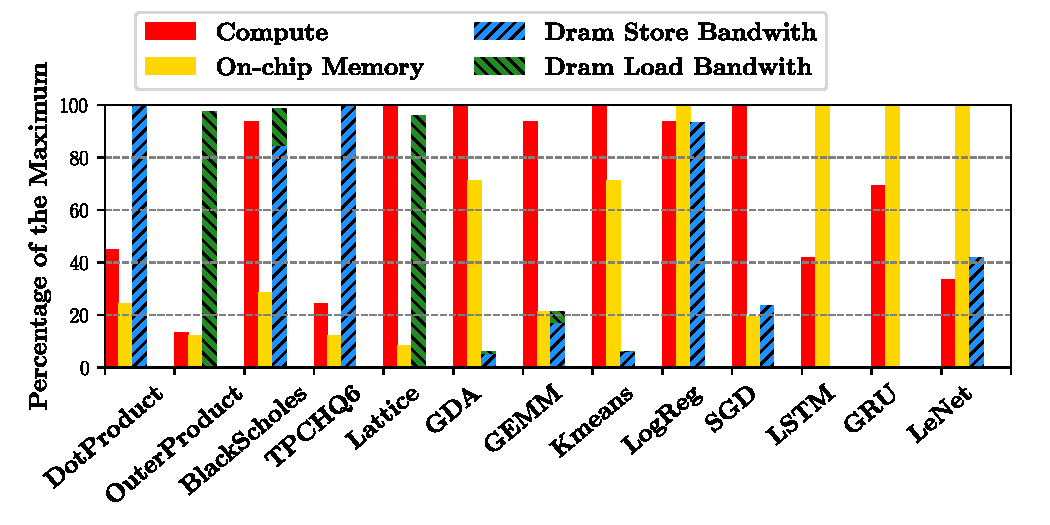
\includegraphics[width=1\columnwidth]{figs/util_bw2.pdf}
\caption{Physical resource and bandwidth utilization for various applications.}\label{fig:util_bw}
\centering
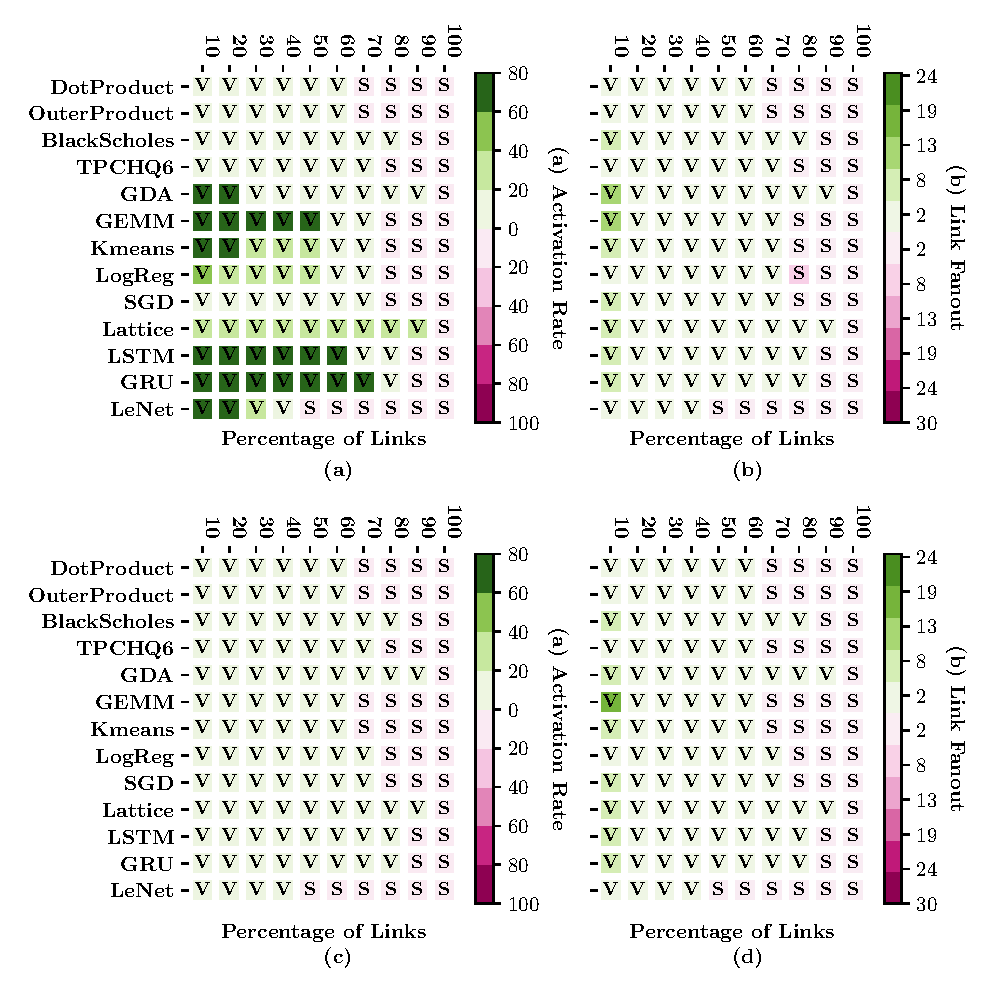
\includegraphics[width=1\columnwidth]{figs/link7.pdf}
  \caption{Application communication patterns on pipelined (a,b) and scheduled (c,d) CGRA architectures.
  (a) and (c) show the activation rate distribution of logical links at runtime. 
  Links sorted by granularity, then rate; darker boxes indicate higher rates.
  The split between green and pink shows the ratio of logical vector to scalar links. (b) and (d) show the distribution of broadcast link fanouts.
 }\label{fig:link}
\end{figure}

\begin{figure}
\centering
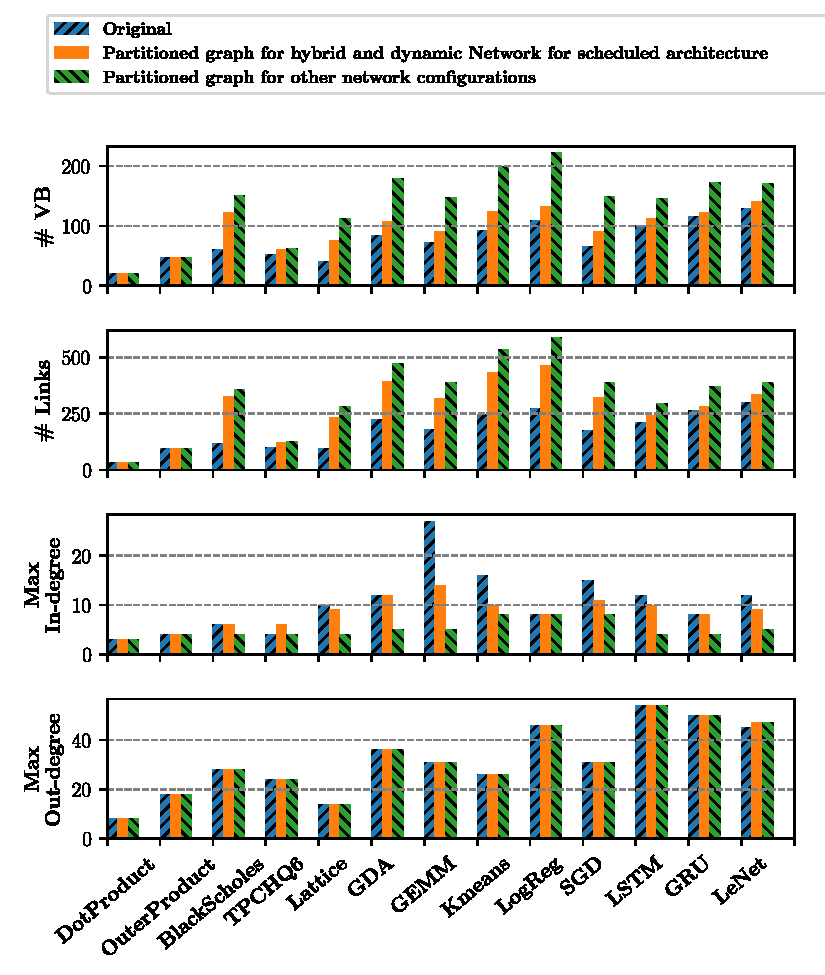
\includegraphics[width=1\columnwidth]{figs/graph.pdf}
\caption{Characteristics of program graphs.}\label{fig:graph}
\end{figure}

We select a mix of applications from domains where hardware accelerators have shown promising performance and energy-efficiency benefits, such as linear algebra, databases, and machine learning.
Table~\ref{tab:benchmark} lists the applications and their data size.
Figure~\ref{fig:util_bw} shows, for each design, which resource limits performance: compute, on-chip memory, or DRAM bandwidth. 
%Variations in these application characteristics introduce different on-chip network requirements.
DotProduct, TPCHQ6, OuterProduct, and BlackScholes are DRAM bandwidth-bound applications. 
These applications use few on-chip resources to achieve maximum performance, resulting in minimal communication.
Lattice (a fast inference model for low-dimensional regression~\cite{garcia2009lattice}), GDA, Kmeans, SGD, and LogReg are compute-intensive applications; for these, maximum performance requires using as much parallelization as possible. 
Finally, LSTM, GRU, and LeNet are applications that are limited by on-chip memory bandwidth or capacity. 
For compute- and memory-intensive applications, high utilization translates to a large interconnection network bandwidth requirement to sustain application throughput. 

Figure~\ref{fig:link}(a,b) shows the communication pattern of applications
characterized on the pipelined CGRA architecture, including the variation in communication granularity. 
Compute and on-chip memory-bound applications show a significant amount of high-bandwidth communication (links with almost 100\% activity). 
A few of these high-bandwidth links also exhibit high broadcast fanout. 
Therefore, a network architecture must provide sufficient bandwidth and efficient broadcasts to sustain program throughput.
On the contrary, time-scheduled architectures, shown in Figure~\ref{fig:link}(c,d), exhibit
lower bandwidth requirements due to the lower throughput of individual compute PUs. 
Even applications limited by on-chip resources have less than a 30\% firing rate on the busiest logical links; this reveals an opportunity for link sharing without sacrificing performance.

Figure~\ref{fig:graph} shows statistics describing the VU dataflow graph before and after partitioning.
The blue bars show the number of VUs, number of logical links, and maximum VU input/output degrees in the original parallelized program; the yellow and green bars show the same statistics after partitioning. 
Fewer VUs are partitioned for hybrid networks and dynamic networks with the time-scheduled architecture, as explained in Section~\ref{sec:partition}. 
The output degree does not change with partitioning because most outputs with a large degree are from broadcast links.


\subsection{Design Space for Network Architectures} \label{sec:network}

We start with several statically allocated network designs, where each SIMD pipeline connects to several switches, and vary flow control strategies and network bisection bandwidth.
In these designs, each switch output connects to exactly one switch input for the duration of the program.
We then explore a dynamic network, which sends program data as packets through a NoC.
The NoC uses a table-based routing scheme at each router to allow for arbitrary routes and tree-based broadcast routing.
Finally, we explore the benefits of specialization by evaluating design points that combine several of these networks to leverage the best features of each.

\subsubsection{Static networks}
We explore static network design points along three axes. 
First, we study the impact of flow-control schemes in static switches. 
In credit-based flow control~\cite{wang2013avoiding}, the source and destination PUs coordinate to ensure that the destination buffer does not overflow.
For this design point, switches only have a single register at each input, and there is no backpressure between switches.
%This design utilizes minimum buffering within switches, but require larger end-point buffering.
%
The alternate design point uses a skid-buffered queue with two entries at each switch; using two entries enables per-hop backpressure and accounts for a one-cycle delay in stalling the upstream switch.
%this is to 
%and take into account for the fact that stall signal will take a cycle to transmit to the nearest switch.
At full throughput, the receiver will consume data as it is sent and no queue will ever fill up.
%this is to account for the difficulty of transmitting a combinational stall signal between multiple switches in a single cycle.
%The stall signal from one stage to the next is only generated if the queue has two entries in it
%The first design point minimizes the number of buffers in the network, which consequently reduces area and energy. 
%However, this scheme requires large end-point buffers to prevent bubbles caused by the round trip credit delay. 
%Skid-buffering alleviates the bubbles with per-hop flow control while consuming twice the amount of buffer area and energy.
%
The second axis studied is the bandwidth, and therefore routability, of the static network. 
We vary the number of connections between switches in each direction, which trades off area and energy for bandwidth.
Finally, we explore specializing static links: using a separate scalar network to improve routability at a low cost.
%As shown in Figure~\ref{fig:link}, a
%significant fraction of communication is scalar. 

\subsubsection{Dynamic networks}
Our primary alternate design is a dynamic NoC using per-hop virtual channel flow control. 
Routing and Virtual Channel (VC) assignment are table-based: the compiler performs static routing and VC allocation, 
and results are loaded as a part of the routers' configurations at runtime.
The router has a separable, input-first VC and switch allocator with a single iteration and speculative switch allocation~\cite{dallytowles}.
Input buffers are sized just large enough (3 entries) to avoid credit stalls at full throughput.
%For some design points, we use a novel heterogeneous VC buffering scheme, with mixed flit widths; in this case, only one VC is capable of handling a full-width (512bit) flit and the others use smaller flits. 
%This allows us to assign links to VCs and maintain freedom from deadlock, while avoiding the area requirements of keeping large, mostly unused buffers.
Broadcasts are handled in the network with duplication occurring at the last router possible to minimize energy and congestion.
To respect the switch allocator's constraints, each router sends broadcasts to output ports sequentially and in a fixed order.
This is because the switch allocator can only grant one output port per input port in every cycle, and the RTL router's allocator does not have sufficient timing slack to add additional functionality.
We also explore different flit widths on the dynamic network, with a smaller bus taking multiple cycles to transmit a packet.

%\subsubsection{VC Allocation for Deadlock Avoidance} 
%Deadlock is a system pathology that occurs when multiple actors hold resources while waiting for each other's resources to become available.
%In a NoC, the actors are flits, and the held/waited-for resources are buffers.
%There are four necessary conditions for permament deadlock \cite{coffman1971system}:
%\begin{enumerate}
%  \item resources are mutually exclusive,
%  \item actors hold resources while waiting on other resources,
%  \item actors can not be preempted, and
%  \item actors wait on each other in a cyclic graph.
%\end{enumerate}

%In traditional NoC designs, there are two types of deadlock: deadlock within a network (such as that from cyclic paths), and \emph{protocol deadlock}.
%These designs are typically based around a request-response model: to avoid protocol deadlock, a node issuing a request will always be ready to receive its response. 
%Then, to ensure that the protocol graph is acyclic, the responses are prevented from waiting indefinitely on resources held by requests by partitioning all buffers in the network into two classes.
%Deadlock within a network is avoided by a variety of schemes, many of which (dateline VC allocation, dimension-order routing) work by imposing restrictions on which holds/waits relationships are valid.
%These restrictions ensure that the full potential holds/waits graph is acyclic, and therefore any subgraph must also be acyclic.

%When extending the deadlock model to a CGRA, there are three main types of deadlock that we need to avoid: traditional network deadlock, endpoint buffer deadlock, and through-node deadlock.
%For CGRAs, there are three main types of deadlock that we need to avoid: traditional network deadlock, endpoint buffer deadlock, and through-node deadlock.
%A key difference between CGRA and CPU networks is that CGRAs operate in a streaming fashion---each spatially distributed node, after completing its assigned work, sends the result to the next node(s).
Because CGRA networks are streaming---each PU pushes the result to the next PU(s) without explicit request---the network cannot handle routing schemes that may drop packets; otherwise, application data would be lost.
%Due to spatial accelerator tends to optimize for lightweight control to maximize compute density, there is also less leverage on complicated routing hardware with packet reordering. 
Because packet ordering corresponds directly to control flow, it is also imperative that all packets arrive in the order they were sent; this further eliminates adaptive or oblivious routing from consideration.
We limit our study of dynamic networks to statically placed and routed source routing due to these architectural constraints.
PUs propagate backpressure signals from their outputs to their inputs, so they must be considered as part of the network graph for deadlock purposes~\cite{hansson2007avoiding}.
Furthermore, each PU has fixed-size input buffers; these are far too small to perform high-throughput, end-to-end credit-based flow control in the dynamic network for the entire program \cite{wang2013avoiding}.
%This is similar to work done on streaming NoCs, where multiple streams of traffic compete for the same resources \cite{hansson2007avoiding, wang2013avoiding}.
%Furthermore, because a compute node must be able to send its output to read its inputs, dependences may be propagated backwards through the network; this means that dimension order routing alone is insufficient to make progress and separate virtual networks must be used.
%\subsubsection{Endpoint Buffer Deadlock}
%This is a type of protocol deadlock that results from head-of-line blocking and finite buffer sizes at node inputs, as shown in Figure~\ref{fig:deadlock}(a).
%Consider two streams, A and B, that traverse the same virtual channel but are destined for different input buffers at the same destination node.
%If A fills up its input buffer, and B's input buffer is empty, the node cannot make progress.
%Simultaneously, if a flit from stream A is at the head of the shared virtual channel, then no flits from stream B will be able to pass it.
%
%At the final hop of the network, this would be trivial to resolve: the final router can use its knowledge of the buffer state of the destination to avoid overloading any single input buffer.
%However, it could be too late to resolve this problem at the final router, because if it blocks the faster flow, and they share a network resource earlier, the slower flow could be head-of-line blocked earlier in the network.
%\subsubsection{Through-Node Deadlock}
%Because nodes do not have infinite buffers, the deadlock graph for a network no longer begins and ends at the routes---it must be extended with information about the program nodes \cite{hansson2007avoiding}.
%%This means that traditional deadlock avoidance techniques, such as dimension-order routing, are \emph{not sufficient} to prevent deadlock in these networks.
%An example of how this can cause deadlock in a y-first dimension-order routed network is shown in Figure~\ref{fig:deadlock}(b).
%This type of deadlock can also combine with endpoint deadlock, in addition to traditional network deadlock.
%Because nodes propagate holds/waits dependences, any indirect input to the final node is capable of creating an endpoint buffer deadlock at the final node with any other indirect input, anywhere in the network.
%When different branches of the tree are fed by different DRAM accesses, one will almost certainly run faster and inevitably lead to this deadlock condition.
Practically, this means that no two logical paths may be allowed to conflict at \emph{any} point in the network; to meet this guarantee, VC allocation is performed to ensure that all logical paths traversing the same physical link are placed into separate buffers.
%Because there are only a finite number of VCs at each router, this is another network constraint to optimize: routes are penalized for exceeding the maximum, which leads to them being moved and a better solution being found.

\subsubsection{Hybrid networks}
Finally, we explore hybrids between static and dynamic networks that run each network in parallel. 
During static place and route, the highest-bandwidth logical links from the program graph are mapped onto the static network; once the static network is full, further links are mapped to the dynamic network.
By using compiler knowledge to identify the relative importance of links---the link fanout and activation factor---hybrid networks can sustain the throughput requirement of most high-activation links while using the dynamic network for low-activation links.
%We place and route our applications to minimize the load on the dynamic network, but we enforce a strict mutual exclusion constraint: a route must be either fully mapped to the dynamic network, or fully mapped to the static network, including broadcast routes.
%This eliminates coordination between networks, and greatly simplifies the mapping problem. It also simplifies the problem of hardware design, because the static network does not need additional crossbar ports to connect to the dynamic network and vice versa.

\subsection{Performance, Area, and Energy Modeling} \label{sec:net_char}

\subsubsection{Simulation}
We use a cycle-accurate simulator to model the pipeline and scheduling delay for the two types of architectures,
 integrated with DRAMSim \cite{dramsim} to model DRAM access latency. For static networks, we model
a distance-based delay for both credit-based and per-hop flow control. 
For dynamic networks, we integrate
our simulator with Booksim \cite{jiang2013detailed}, adding support for arbitrary source routing using look-up tables. 
Finally, to support efficient multi-casting in the dynamic network, we modify Booksim to duplicate broadcast packets at the router where their paths diverge.
At the divergence point, the router sends the same flit to multiple output ports over multiple cycles.
We assume each packet carries a unique ID that is used to look up the output port and next VC in a statically generated routing table, and that the ID is roughly the same size as an address.
When the packet size is greater than the flit size, the transmission of a single packet takes multiple cycles.
%\info{is it worth mentioning how large flit are transmitted on small flit routers? are they just treated as packet?}
%We simulate the priority VC functionality by determining which packets will traverse non-priority VCs using the generated placement.
%These packets are scaled, to account for the smaller effective flit size and therefore the need to send multiple flits.

\begin{table*}
\centering
  \footnotesize
  \begin{tabular*}{6.25in}{p{0.75in} p{3in} p{2.5in}}
    \bottomrule
    \textbf{Benchmark} & \textbf{Description} & \textbf{Data Size} \\ \midrule
    DotProduct & Inner product & $1048576$ \\ \midrule
    OuterProduct & Outer product &$1024$ \\ \midrule
    BlackScholes & Option pricing &$1048576$ \\ \midrule
    TPCHQ6 & TPC-H query 6 &$1048576$ \\ \midrule
    Lattice & Lattice regression~\cite{garcia2009lattice} &$1048576$\\ \midrule
    GDA & Gaussian discriminant analysis &$127\times1024$ \\ \midrule
    GEMM & General matrix multiply &$256\times256\times256$ \\ \midrule
    Kmeans & K-means clustering &k=64, dim=64, n=8192, iter=2 \\ \midrule
    LogReg & Logistic regression &$8192\times128$, iter=4\\ \midrule
    SGD & Stochastic gradient descent for a single layer neural network &$16384\times64$, epoch=10 \\ \midrule
    LSTM & Long short term memory recurrent neural network &1 layer, 1024 hidden units, 10 time steps \\ \midrule
    GRU & Gated recurrent unit recurrent neural network &1 layer, 1024 hidden units, 10 time steps \\ \midrule
    LeNet & Convolutional neural network for character recognition& 1 image\\ \midrule
  \end{tabular*}
  \caption{Benchmark summary}
  \label{tab:benchmark}
\end{table*}


\subsubsection{Area and power}
% Elaborate more here since reviewers were confused
To efficiently evaluate large networks, we start by characterizing the area and power consumption of individual routers and switches
used in various network configurations. 
The total area and energy are then aggregated over all switches and routers in a particular network.
We use router RTL from the Stanford open source NoC router \cite{becker2012efficient} and our own parameterized switch implementation.
We synthesize using Synopsys Design Compiler with a \SI{28}{nm} technology library and clock-gating enabled, meeting timing at a 1 GHz clock frequency.
%For both the switch and the router, we enable clock-gating during synthesis to reduce dynamic power. 
Finally, we use Synopsys PrimeTime to back-annotate RTL signal activity to the post-synthesis switch and router designs to estimate gate-level power.

We found that power consumption can be broken into two types: 
inactive power consumed when switches and routers are at zero-load ($P_{\text{inactive}}$, which includes both dynamic and static power),
and active power. The active power, as shown in Section~\ref{sec:net_char}, is proportional to the amount of
data transmitted. 
Because power scales linearly with the amount of data movement, we model the marginal energy to transmit a single flit of data (flit energy, $E_{\text{flit}}$) by dividing active energy by the number flits transmitted in the testbench:
\begin{equation}
  E_{\text{flit}} = \frac{\left(P-P_{\text{inactive}}\right) T_{\text{testbench}}}{\#\text{flit}} 
\end{equation}
While simulating an end-to-end application, we track the number of flits transmitted at each switch and router in the network, as well as the number of switches and routers allocated by place and route. 
We assume unallocated switches and routers are perfectly power-gated, and do not consume energy.
The total network energy for an application on a given network ($E_{\text{net}}$) can be computed as:
\begin{equation}
  E_{\text{net}} = \sum_{\text{allocated}} P_{\text{inactive}} T_{\text{sim}}
  + E_{\text{flit}}  \#\text{flit},
\end{equation}
where $P_{\text{inactive}},$ $E_{\text{flit}},$ and $\#\text{flit}$ are tabulated separately for each network resource.

%we model the energy needed to transmit a single flit through 
%the designs by using linear regression to separate power consumed when no flits are transmitted (e.g., clock network power) and power consumed when flits are transmitted.
%We assume unused switches and routers can be power gated, and we enable clock gating to reduce dynamic power when network is idle.
%The total network energy of an application on a given network design point is composed of zero-load power for switches and routers that cannot be power gated, and per-flit power for each network communication.

\begin{figure}
\centering
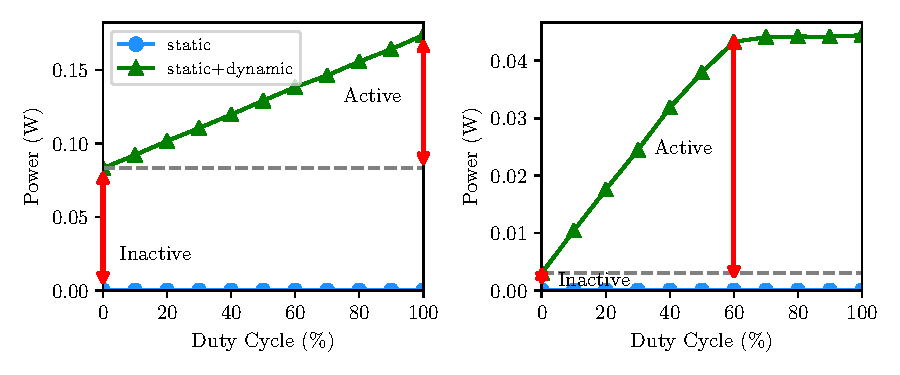
\includegraphics[width=1\columnwidth]{figs/sweep.pdf}
  \caption{Switch and router power with varying duty cycle.}\label{fig:sweep}
\end{figure}


Figure~\ref{fig:sweep} shows that switch and router power scale linearly with the rate of data transmission, but that there is non-zero power at zero-load. 
For simulation, the duty cycle refers to the amount of offered traffic, not accepted traffic.
Because our router uses a crossbar without speedup \cite{dallytowles}, the testbench saturates the router at 60\% duty cycle when providing uniform random traffic. 
Nonetheless, router power still scales linearly with accepted traffic.

A sweep of different switch and router parameters is shown in Figure~\ref{fig:char}. Subplots (d,e,f) show the energy necessary to transmit a single bit through a switch or router.
Subplot (a) shows the roughly quadratic scaling of switch area with the number of links between adjacent switches.
Vector switches scale worse with increasing bandwidth than scalar switches, mostly due to increased crossbar wire load. 
At the same granularity, a router consumes more energy a switch to transmit a single bit of data, even though the overall router consumes less power (as shown in Figure~\ref{fig:sweep}); 
this is because the switch has a higher throughput than the router.
The vector router has lower per-bit energy relative to the scalar router because it can amortize the cost of allocation logic, whereas the vector switch has higher per-bit energy relative to the scalar switch due to increased capacitance in the large crossbar. 
Increasing the number of VCs or buffer depth per VC also significantly increases router area and energy, but reducing the router flit width can significantly reduce router area. 

\begin{figure}
\centering
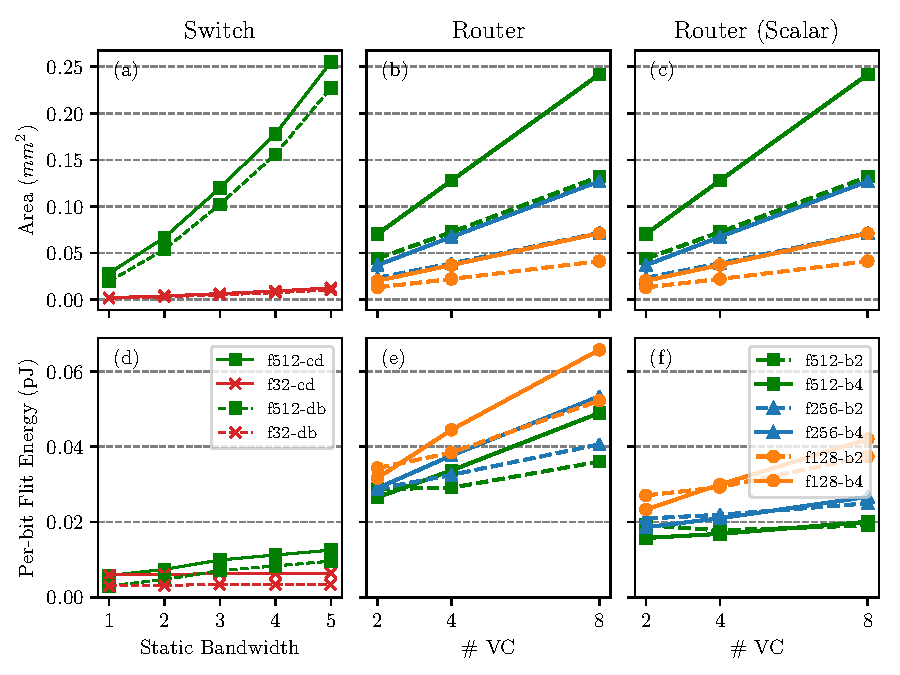
\includegraphics[width=1\columnwidth]{figs/char.pdf}
  \caption{Area and per-bit energy for (a,d) switches and (b,c,e,f) routers. 
  (c,f) Subplots (c,f) show area and energy of the vector router when used for scalar values (32-bit).}\label{fig:char}
\end{figure}

Overall, these results show that scaling static bandwidth is cheaper than scaling dynamic bandwidth, and a dynamic network with small routers can be used to improve link sharing for low bandwidth communication.  
We also see that a specialized scalar network, built with switches, adds negligible area compared to and is more energy efficient than the vector network. 
Therefore, we use a static scalar network with a bandwidth of 4 for the remainder of our evaluation, except when evaluating the pure dynamic network.
The dynamic network is also optimized for the rare instances when the static scalar network is insufficient. 
When routers transmit scalar data, the high bits of data buffers are clock-gated, reducing energy as shown in (f).
Figure~\ref{fig:area} summarizes the area breakdown of all the network configurations that we evaluate.

\begin{figure}
\centering
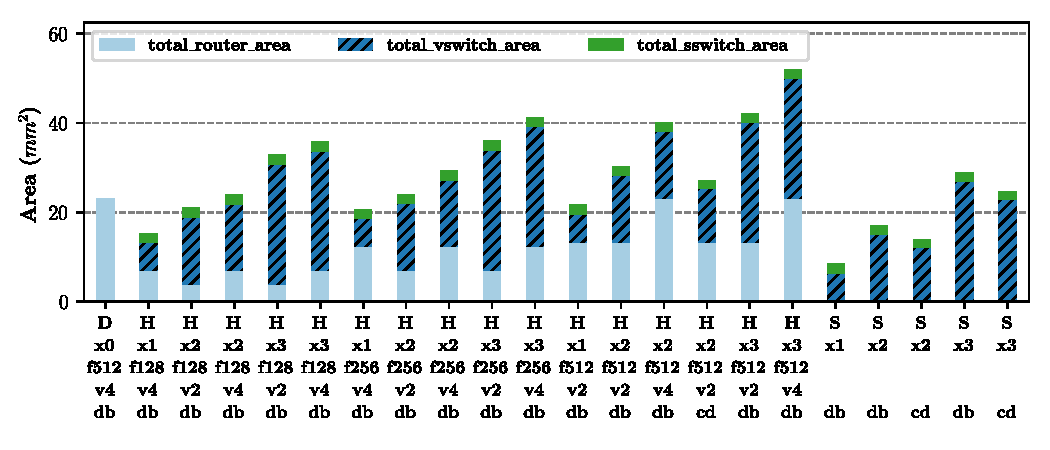
\includegraphics[width=1\columnwidth]{figs/area.pdf}
  \caption{Area breakdown for all network configurations.}\label{fig:area}
\end{figure}

\subsection{Network Architecture Evaluation} \label{sec:net_dse}

\begin{table}
\footnotesize
\begin{tabular*}{\columnwidth}{p{1cm} p{7cm}}
  \bottomrule
  \textbf{Notation} & \textbf{Description} \\\midrule
  $[$S,H,D$]$ & Static, hybrid, and dynamic network \\\midrule
  x\# & Static bandwidth on vector network (\#links between switches) \\\midrule
  %$s\#$ & Number of links between switches on static scalar network \\\midrule
  f\# & Flit width of a router or vector width of a switch \\\midrule
  v\# & Number of VC in router \\\midrule
  b\# & Number of buffers per VC in router \\\midrule
  $[$db,cd$]$ & Buffered vs. credit-based flow control in switch \\\midrule
  %$[Scheduled, Pipelined]$ & Time scheduled vs deep pipelined accelerator architectures \\\midrule
\end{tabular*}
\caption{Network design parameter summary.}
\label{tab:notation}
\end{table}
We evaluate our network configurations in five dimensions: performance (perf), performance per network area (perf/area), performance per network
power (perf/watt), network area efficiency (1/area), and network power efficiency (1/power). 
Among these metrics, performance is the most important: networks only consume a small fraction of the overall accelerator area and energy (roughly 10-20\%). 
Because the two key advantages of hardware accelerators are high throughput and low latency, 
we filter out a network design point if it introduces
more than 10\% performance overhead.
This is calculated by comparing to an ideal network with infinite bandwidth and zero latency.

For metrics that are calculated per application, such as performance, performance/watt, and power efficiency, we first normalize the metric with respect to the 
worst network configuration for that application. 
For each network configuration, we present a geometric mean normalized across all applications. 
For all of our experiments, except Section~\ref{sec:scale}, we use a network
size of $14\times14$ end-point PUs. All vector networks use a vectorization factor of 16 (\SI{512}{bit} messages).

\begin{figure}
\centering
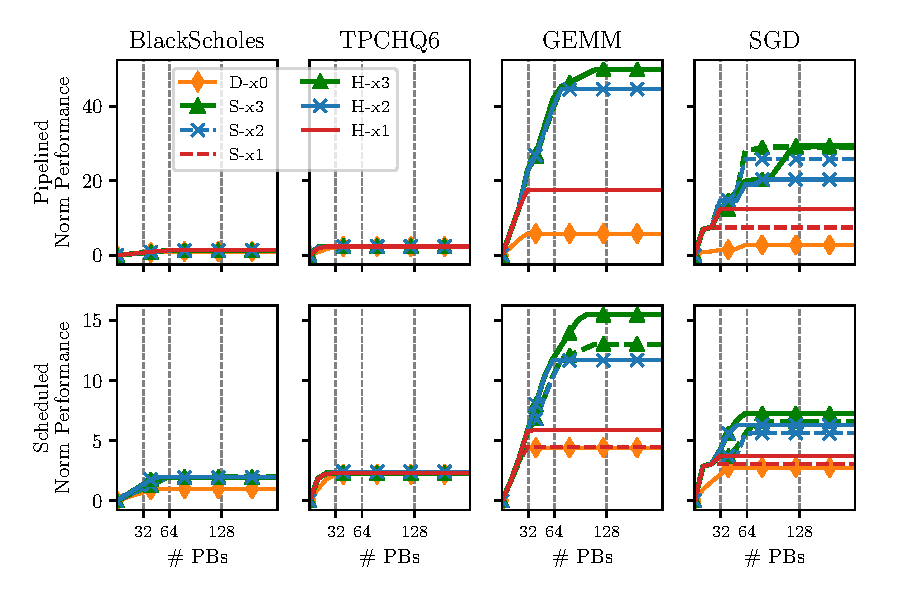
\includegraphics[width=1\columnwidth]{figs/scale.pdf}
\caption{Performance scaling with increased CGRA grid size for different networks.}\label{fig:scale}
\end{figure}
\subsubsection{Bandwidth scaling with network size}\label{sec:scale}
%Figure~\ref{fig:scale} shows the performance scaling of applications as accelerator size scales with different network configurations.
Figure~\ref{fig:scale} shows how different networks allow several applications to scale to different numbers of PUs.
For IO-bound applications (BlackScholes and TPCHQ6), performance does not scale with additional compute and on-chip memory resources.
However, the performance of compute-bound applications (GEMM and SGD) improves with increased resources, but plateaus at a level that is determined by on-chip network bandwidth. 
%Although this is expected for general network designs, it is much more noticeable due to the high-bandwidth communication inherent in pipelined reconfigurable accelerators.
This creates a trade-off in accelerator design between highly vectorized compute PUs with a small network---which would be underutilized for non-vectorized problems---and smaller compute PUs with limited performance due to network overhead. 
For more finely grained compute PUs, both more switches and more costly (higher-radix) switches must be employed to meet application requirements.

The scaling of time-scheduled accelerators (bottom row) is much less dramatic than that of deeply pipelined architectures (top row). 
Although communication between PUs in these architectures is less frequent, the scheduled architecture must use additional parallelization to match the throughput of the pipelined architecture; this translates to larger network sizes. 
%Since scaling dynamic bandwidth is much more expensive than scaling static bandwidth, as shown in section \ref{sec:net_char}, 
%we only explored scaling bandwidth in vector switches. 

For pipelined architectures, both hybrid and static networks provide similar scaling with the same static bandwidth:
the additional bandwidth from the dynamic network in hybrid networks does not provide additional scaling. 
This is mostly due to a bandwidth bottleneck between a PU and its router, which prevents the PU from requesting multiple elements per cycle.
Hybrid networks tend to provide better scaling for time-scheduled architectures; multiple streams can be time multiplexed at each ejection port without losing performance.

\begin{figure}
\centering
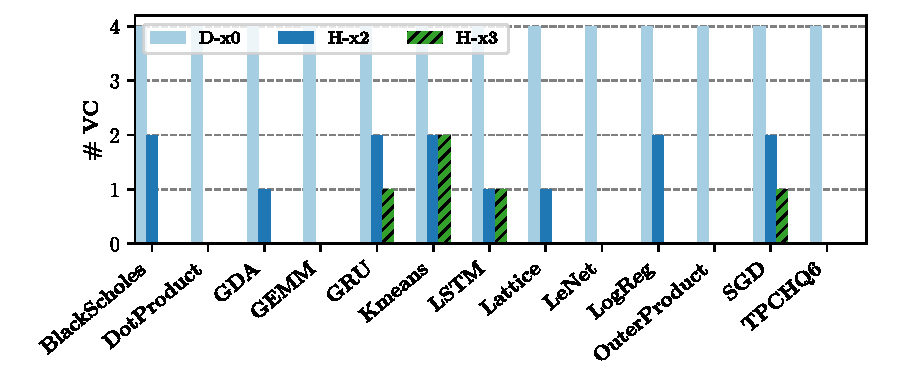
\includegraphics[width=1\columnwidth]{figs/vc.pdf}
  \caption{Number of VCs required for dynamic and hybrid networks. (No VCs indicates that all traffic is mapped to the static network.)}\label{fig:vc}
\end{figure}

\begin{figure}
  \centering
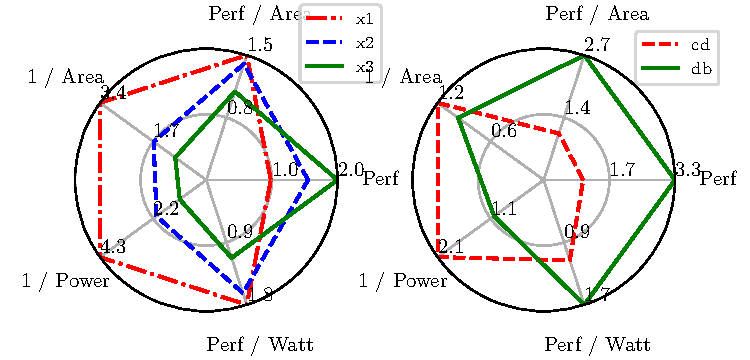
\includegraphics[width=0.8\columnwidth]{figs/radar_switch.pdf}
  \caption{
    Impact of bandwidth and flow control strategies in switches.}\label{fig:radar_switch}
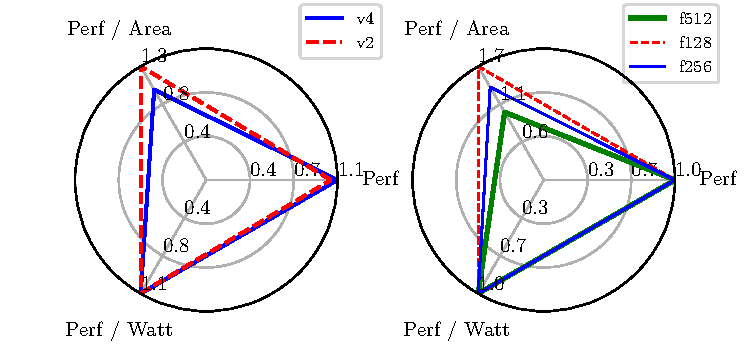
\includegraphics[width=0.8\columnwidth]{figs/radar_router.pdf}
  \caption{Impact of VC count and flit widths in routers.}\label{fig:radar_router}
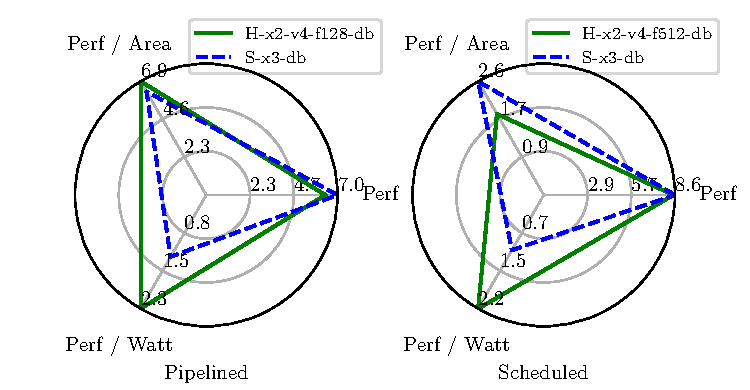
\includegraphics[width=0.8\columnwidth]{figs/radar_best.pdf}
  \caption{Geometric mean improvement for the best network configurations, relative to the worst configuration.}\label{fig:radar_best}
\end{figure}

\begin{figure*}
\centering
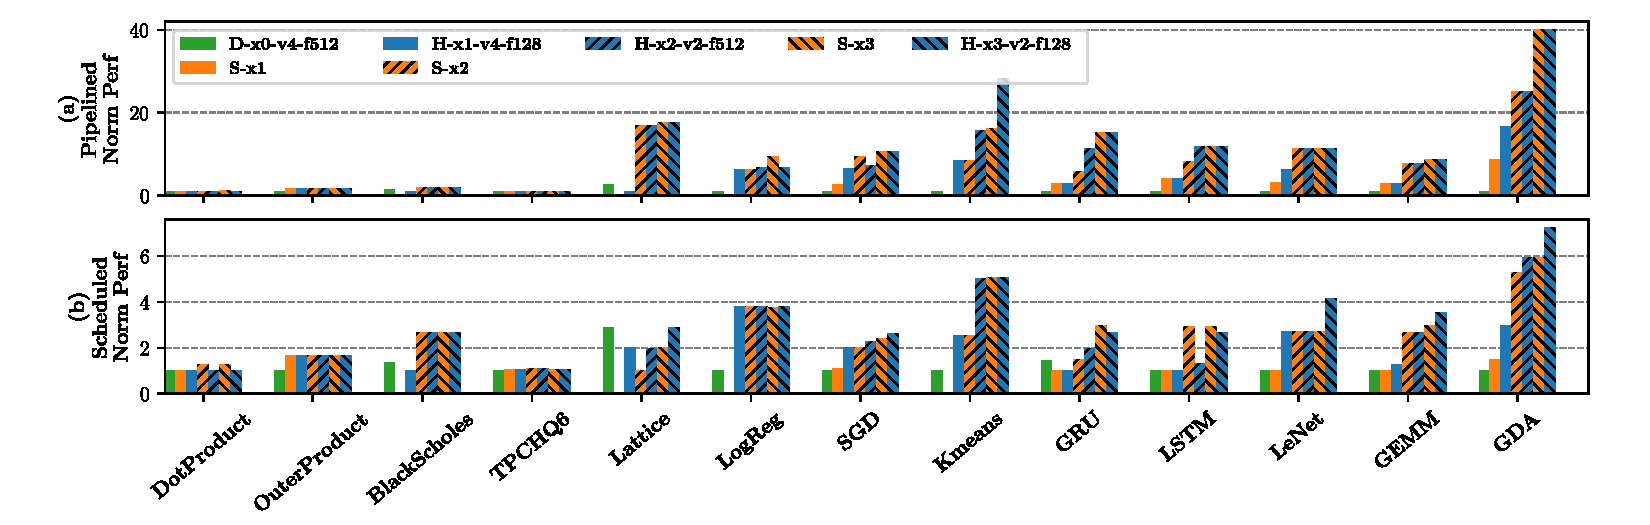
\includegraphics[width=1\linewidth]{figs/perf.pdf}
  \caption{Normalized performance for different network configurations.}\label{fig:perf}
\end{figure*}

\begin{figure}
\centering
  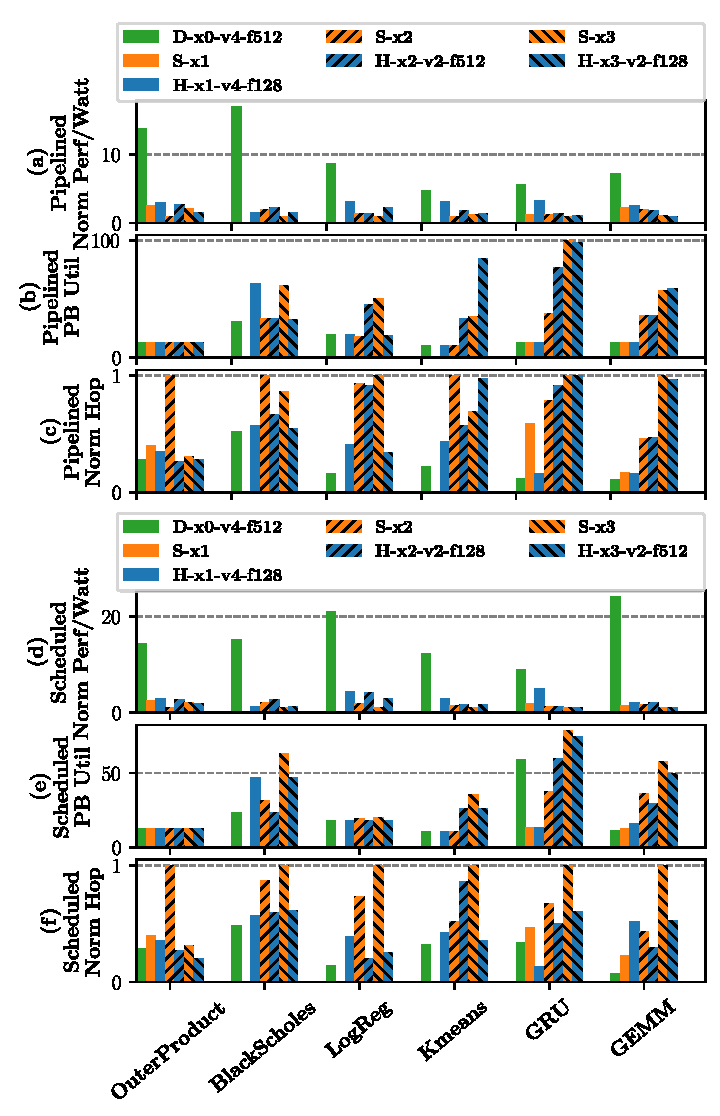
\includegraphics[width=0.8\columnwidth]{figs/energy.pdf} 
\caption{(a,d): Normalized performance/watt. (b,e): Percentage of compute and memory PUs utilized for each network configuration. 
  (c,f): Total data movement (hop count).}
\label{fig:energy}
\end{figure}

\subsubsection{Bandwidth and flow control in switches}

In this section, we study the impact of static network bandwidth and flow control mechanism (per-hop vs. end-to-end credit-based). 
On the left side of Figure~\ref{fig:radar_switch}, we show that increased static bandwidth results in a linear performance increase and a superlinear increase in area and power. 
As shown in Section~\ref{sec:scale}, any increase in accelerator size must be coupled with increased network bandwidth to effectively scale performance. 
This indicates that network overhead will increase with the size of an accelerator.

The right side of Figure~\ref{fig:radar_switch} shows that, although credit-based flow control reduces the amount of buffering in switches and decreases network area and energy, application performance is significantly impacted. 
This is the result of imbalanced data-flow pipelines in the program: when there are parallel long and short paths over the network, there must be sufficient buffer space on the short path equal to the product of throughput and the difference in latency. 
Because performance is our most important metric, credit-based flow control is not feasible, especially because the impact of bubbles increases with communication distance, and therefore network size.

\subsubsection{VC count and reduced flit width in routers}
In this experiment, we study the area-energy-performance trade-off between routers with different VC counts. As shown
in Section~\ref{sec:net_char}, using many VCs increases both network area and energy.
However, using too few VCs may force roundabout routing on the dynamic network or result in VC allocation failure when the network is heavily utilized.
Nonetheless, the left side of Figure~\ref{fig:radar_router} shows minimal performance improvement from using more VCs. 

Therefore, for each network design, we use a VC count equal to the maximum number of VCs required to map all applications to that network. 
Figure~\ref{fig:vc} shows that the best hybrid network configurations with 2x and 3x static bandwidth require at most 2 VCs, whereas the pure dynamic network requires 4 VCs to map all applications.
%This is different from a traditional processor based (request-response) architecture because, first, less VCs are required to map a large amount of traffic onto dynamic network due deadlock challenges
%specific to streaming architectures, second, communication is much infrequent to incur bandwidth penalty on dynamic network. 
Because dynamic network communication is infrequent, hybrid networks with fewer VCs provide both better energy and area efficiency than networks with more VCs, even though this constrains routing on the dynamic network.
%The improvement is less significant in a time-scheduled architecture because of an overall reduction in required bandwidth.

We also explore the effects of reducing dynamic network bandwidth by using smaller routers;
as shown in Section~\ref{sec:net_char}, routers with smaller flits have a much smaller area.
Ideally, we could scale static network bandwidth while using a low-bandwidth router to provide an escape path and reduce overall area and energy overhead. 
The right side of Figure~\ref{fig:radar_router} shows that, for a hybrid network, reducing flit width improves area efficiency with minimal performance loss. 

%The reduction in performance is more significant in pipelined CGRAs than time-scheduled CGRAs, as the latter has a lower bandwidth requirement.

\subsubsection{Static vs. hybrid vs. dynamic networks}

Figure~\ref{fig:perf} shows the normalized performance for each application running on several network configurations.
%For some applications, the ideal configuration could not be placed and routed onto a static network with 1x bandwidth; missing bars for S-x1 are the result of these failures.
For some applications, the bar for S-x1 is missing; this indicates that place and route failed for all unrolling factors.
For DRAM-bound applications, the performance variation between different networks is trivial because only a small fraction of the network is being used. 
In a few cases (Kmeans and GDA), hybrid networks  provide better performance due to slightly increased bandwidth.
For compute-bound applications, performance primarily correlates with network bandwidth because more bandwidth permits a higher parallelization factor. 

%Figures~\ref{fig:energy} [1,4] show the normalized performance/watt of the network for pipelined and scheduled
%architectures. Figure [2,5] show the corresponding PU utilizations in the network. Figure [3,6] summarize the total
%data movement distributed on static vector, static scalar, dynamic vector and dynamic scalar for that network
%configuration.  
The highest bandwidth static network uses the most PUs, as shown in Figures~\ref{fig:energy}(b,e), because it permits more parallelization. 
It also has more data movement, as shown in (c,f), because PUs can be distributed farther apart. 
Due to bandwidth limitations, low-bandwidth networks perform best with small unrolling factors---they are unable to support the bisection bandwidth of larger program graphs.
This is evident in Figures~\ref{fig:energy}(b,e), where networks D-x0-v4-f512 and S-x2 have small PU utilizations.

With the same static bandwidth, most hybrid networks have better energy efficiency than the corresponding pure static networks, even though routers take more energy than switches to transmit the same amount of data.
This is a result of allowing a small amount of traffic to escape onto the dynamic network: with the dynamic network as a safety net, static place and route tends to converge to better placements with less overall communication.
This can be seen in Figures~\ref{fig:energy}(c,f), where most static networks have larger hop counts than the corresponding hybrid network; hop count is the sum of all runtime link traversals, normalized per-application to the network configuration with the most hops.
Subplots (e,f) show that more PUs are utilized with static networks than hybrid networks.
%Compared to hybrid networks, (e,f), show larger PU utilization at the same parallelization factor on the purely static network .
This is because the compiler imposes less stringent IO constraints on PUs when partitioning for the hybrid network (as explained in Section~\ref{sec:partition}), which results in fewer PUs, less data movement, and greater energy efficiency for hybrid networks.

In Figure~\ref{fig:radar_best}, we summarize the best perf/watt and perf/area (among network configurations with <10\% performance overhead) for pipelined and scheduled CGRA architectures. 
Pure dynamic networks are not shown because they perform poorly due to insufficient bandwidth.
On the pipelined CGRA, the best hybrid network provides a 6.4x performance increase, 2.3x better energy efficiency, and a 6.9x perf/area increase over the worst network configuration. 
The best static network provides 7x better performance, 1.2x better energy efficiency, and 6.3x better perf/area. 
The hybrid network gives the best perf/area and perf/watt, with a small degradation in performance when compared to the static network. 
On the time-scheduled CGRA, both static and hybrid networks have an 8.6x performance improvement. 
The hybrid network gives a higher perf/watt improvement at 2.2x, whereas the static network gives a higher perf/area improvement at 2.6x.
Overall, the hybrid networks deliver better energy efficiency with shorter routing distances by allowing an escape path on the dynamic network.

%It can also provide a decent area efficiency when coupled with a small dynamic network with a minimum performance penalty. 

%\begin{figure}[ht]
%\centering
%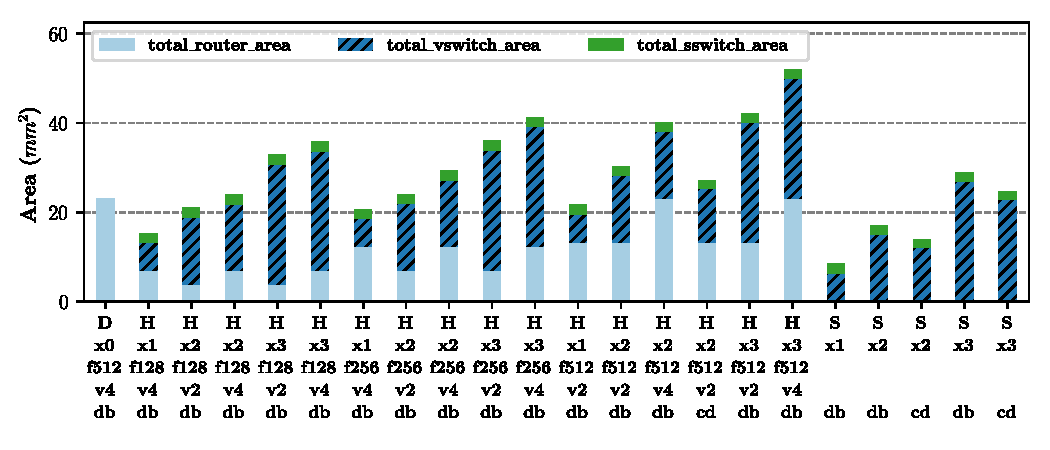
\includegraphics[width=\columnwidth]{figs/area.pdf}
%\caption{Area breakdown of network architectures}\label{fig:area}
%\end{figure}

%In this section, we evaluate the proposed network architecture design points from Section~\ref{sec:network}, summarized in Table~\ref{tab:net_dse}.
%Pure dynamic networks are represented with $D{\dash}v0{\dash}s0$, indicating no static links in the network. 
%Pure static networks are prefixed with $v\#{\dash}s\#$, where the $\#$ are number of
%scalar and vector links between switches. Hybrid networks are shown as $D{\dash}v\#{\dash}s\#$.
%Figure~\ref{fig:area_vc} (a) shows the number of VCs required to map each application for architectures containing a dynamic network. 
%%The maximum number of VCs required across all applications is the number of VCs we use to account for area. 
%When computing area for each configuration, we use the maximum number of VCs required to map any application.
%For application in hybrid network with no VCs, all traffic is mapped onto the static network.

%Figure~\ref{fig:area_vc} (b) shows the area breakdown of the architecture. 
%For $D{\dash}v0{\dash}s0$, all links are routed through the dynamic network, resulting in heavy congestion and a large VC requirement. 
%Consequently, the large number of VCs directly contribute to the large router area. 
%All the other dynamic configurations only need 2 VCs to avoid deadlock. 
%The network area contributes only a small fraction of the overall area, but using a dynamic network with a smaller flit width saves router area roughly linearly.
%%The hybrid network $D{\dash}v1{\dash}s4-f512, and D{\dash}v2{\dash}s4-f512$ has slightly larger area than their equivalent bandwidth counterpart design point in static network $v2{\dash}s4$ and $v3{\dash}s4$ due to the overhead on dynamic routing and buffering. 

%Figure~\ref{fig:slow_down} (a) shows the performance degradation normalized to the ideal network with infinite buffers; all the other design points have an end-point buffer with depth 4 inside the CUs.
%We found that for memory bandwidth bound applications, the performance is roughly the same across all design points, mostly due to the low CU utilization and lack of congestion. 
%Although BlackScholes is DRAM bandwidth bound, the inner loop partition introduces lots of CUs communicating their temporary results. 
%The slow-down with BlackScholes with static network compared to ideal network is due to the pipeline bubbles introduced by VU partitioning as explained in Section \ref{sec:network}. 

%Overall, the hybrid network with the $v1$ static network has a slowdown of less than 2x overall, while the hybrid network with $v2$ has static-equivalent performance.

%The static network with credit-based flow control suffers from insufficient end-point buffers for most applications, resulting in poor performance. 
%The slowdown in dynamic and hybrid networks is mostly due to the high-throughput broadcasts and congestion. 
%Figure~\ref{fig:slow_down} (b) shows the slowdown normalized to total area. 
%Since the network only takes a small fraction of the chip area, the trends is similar to performance. 

%Figure~\ref{fig:slow_down}(c) shows the network energy normalized to $v2{\dash}s4$. 
%The pure dynamic network consumes the most energy because of the amount of buffers and the router's inherently higher per-flit energy. 
%Breaking down the hybrid network energy, we can see that vast majority of communication is mapped to the static network. 
%There is a small gap between energy on $v2{\dash}s4$ and $D{\dash}v2{\dash}s4$, where the hybrid consumes less energy, even though all traffic is mapped onto the static network. 
%Another outlier on LeNet $D{\dash}v2{\dash}s4$ consumes more energy then $v2{\dash}s4{\dash}db$ is likely introduced by randomness from the iterative placer. 
%These are discrepancies introduced by different placements having different distances between nodes.
%It is also important to note hat the overprovisioned static capacity has a high (31\%) mean energy cost, even though it is not being used.
%%This is due to a limitation in current implementation that pure static networks are placed and routed with only back tracking placer, while the hybrid is also using the iterative placer. 
%%As a result, we found better mapping on hybrid network which reduce the hop distance on links, which is not essential for slowdown but directly translates into energy. 
%%However, in theory we should be able to use both algorithm on all design points. 

%In Figure~\ref{fig:slow_down} (d), we show the normalized power. 
%Here, design points with large slowdown naturally have lower power, such as $v3{\dash}s4{\dash}cd$. 
%However, we also show that the network is consuming only a very small portion of the power compared with the compute tiles. 
%The network only consumes around 0--3 W of energy compared to the theoretical peak Plasticine power of 49W.
%Therefore, among the metrics of performance, area, and power, performance is the most important metric to measure the network architectures. 

%%
%%This allows it to be stored in the smaller buffers without any translation logic, and does not result in a loss of throughput (the throughput would be limited regardless at the non-priority VC).
%%Because the priority VC is considered in route scoring, the placer is able to ensure that less than 1\% of traffic in the worst app (XXX) traverses non-priority VCs.
%%This scheme results in a XXX\% lower network area, with a geometric mean slowdown of XXX\% (worst XXX\%).
